\documentclass[10pt, a4paper]{article}
\usepackage[spanish]{babel}
\usepackage[utf8]{inputenc}
\usepackage{graphicx}
\usepackage{multicol}
\usepackage[pdftex]{hyperref}

\hypersetup{colorlinks,%
	    citecolor=black,%
	    filecolor=black,%
	    linkcolor=black,%
	    urlcolor=blue}

\begin{document}
    \title{An\'alisis Grafol\'ogico.}
    \author{Sheyla Leyva S\'anchez \\ Alejandra Monz\'on Pe\~na \\ Laura Riera \\ Andry Rosquet \\ Kevin Talavera \\ Javier}
    \date{}
    \maketitle

    \begin{abstract}
        La grafología es una técnica que estudia las características psicológicas de las personas a través de su escritura. 
        En algunos centros laborales se utilizan este tipo de análisis para determinar cuando contratar o no a alguien y se emplea también 
        para analizar a criminales y en el prceso de determinar trastornos en personas. Esta tarea realizada por expertos,
        psicólogos y grfólogos, resulta complicada y los resultados están numerosas veces sujetos a la perspectiva de quien los analiza. La propuesta de este trabajo es 
        utilizar algoritmos de Aprendizaje Máquina para automáticamente poder predecir características psicológicas de un individuo a partir de un fragmento de su escritura. 
        Utilizaremos un conjunto de algoritmos de ML como: CNN, SVM y DT a modo comparativo para el análisis grafológico. 
        Se propone la creaci\'on de una base de datos de im\'agenes con escritura a mano, as\'i como su uso para entrenar y comparar algunos modelos de Aprendizaje de M\'aquinas para predecir la personalida bas\'andonos en el Test de los Cinco Grandes(Big Five).
    \end{abstract}
    
    \section{Grafolog\'ia}
    
        La grafología es el análisis de la escritura manuscrita de un individuo con la intención de determinar rasgos de personalidad. 
        No existe evidencia científica que respalde la efectividad de la grafología, por lo que es considerada una pseudociencia 
        y una práctica científicamente cuestionable.\\ 

        Tal y como se menciona en el art\'iculo \cite{19} la grafolog\'ia no se utiliza para predecir el futuro o conocer el pasado de una persona. Su uso 
        est\'a dado como una habilidad para conocer el estado psicol\'ogico de la persona en el momento que escribe, incluso se plantea que los resultado de este an\'alisis 
        puede depender de la edad de la persona o del momento en que redacta; es decir una misma persona puede tener resultados diferentes si se analiza su escritura en dos momentos 
        diferentes de su vida.\\

        Según diversos estudios, si tienes un tamaño de letra grande es probable que seas una persona sociable, valiente y muy segura de ti misma. 
        Por otro lado, si tu letra es mediana, significa que te adaptas fácilmente a las circunstancias y eres abierto al cambio. 
        Por \'ultimo, si escribes con una letra de tamaño pequeño, tiendes a ser tímido, meticuloso e introvertido.\\

        Si el espacio que incluyes entre las letras es amplio, significa que aprecias tu libertad y que no te gusta sentirte abrumado o rodeado por mucha gente. 
        Si es angosto, no te agrada estar solo y prefieres vivir en compañía.\\

        En el art\'iculo \cite{17} analizan los rasgos de escritura con el objetivo de crear perfiles para los asesinos, en este art\'iculo explican que 
        rasgos psicol\'ogicos se vinculan a: Espaciado de palabras, Espaciado de l\'ineas, M\'argenes, Inclinaci\'on, Presi\'on del l\'apiz, Forma de letras i, Forma de letras t, entre otras. \\ 


    
    \section{Grafolog\'ia y Aprendizaje M\'aquina}
    
        La combinaci\'on de Aprendizaje M\'aquina y Grafolog\'ia es abordada en un amplio conjunto de art\'iculos en los que se prueban ideas diversas, e incluso se comparan los resultados obtenidos haciendo uso de
        diferentes t\'ecnicas y combin\'andolas.\\ 

        En los art\'iculos \cite{1} y \cite{2} abordan ideas de preprocesado de las im\'agenes manuscritas haciendo uso del unbral adaptativo Gaussiano y llevando a binario los valores de los p\'ixeles de la im\'agen atendiendo a un
        nivel de tolerancia prefijada.\\ 

        Las Redes Neuronales Convolucionales (CNN) debido a su amplio uso para el trabajo con im\'agenes, en el art\'iculo \cite{1} se usan las CNN como m\'etodo propuesto en la arquitectura de una p\'agina web que permita determinar la personalidad 
        a partir de la escritura. En otros como \cite{3} se emplea este m\'etodo en el an\'alisis de firmas, analizando la inclinaci\'on y el espaciado entre caracteres, con la limitaci\'on de que el dataset utilizado solamente posee 10 firmas de 6 individuos. \\ 

        De igual modo las CNN conjuntamente con Regresi\'on log\'istica se emplearon en \cite{4} para predecir el comportamiento financiero de una persona, en este caso con un dataset de más de 200 muestras de escrituras de un texto dado y resultados de un cuestionario de acuerdo al Big Five Personality Model.\\ 

        Otro algoritmo utilizado para el an\'alisis grafol\'ogico es SVM, empleado en \cite{2}, \cite{5}, \cite{6}, \cite{7} y \cite{8}. En el caso de \cite{6} emplean el algoritmo sobre firmas de 53 participantes, para obtener un 71\% de efectividad, 
        en otros como \cite{5} y \cite{8} se compara con otros algoritmos, en el primero con ANN y DNN y en el segundo con KNN y \'arboles de decisi\'on para predecir los resultados del Big Five, en este art\'iculo se utiliz\'o para el SVM un kernel RBF.\\ 

        Tambi\'en se utilizan: K-Means \cite{9}, Fuzy C-Means \cite{10}, ANN \cite{11,5,12,9}, Random Forest \cite{13, 14} y KNN \cite{14,9,8}.\\

        En el art\'iculo \cite{18} realizan un estado del arte sobre grafolog\'ia y Machine Learning en el cual comparan las investigaciones realizadas en 
        otros art\'iculos respecto a los Features utilizados, las caracter\'isticas del dataset, algoritmo empleado y resultados obtenidos.

    \section{Bases de Datos}

        Las bases de datos utilizadas en los estudios de grafolog\'ia realmente contienen informci\'on escasa. En muchos casos 
        son privadas y para acceder a ellas es necesario pagar. En el art\'iculo \cite{14} muestran una tabla comparativa de los datasets disponibles en 
        internet que se han utilizado en otros art\'iculos, en la misma describen cu\'ales son los tags presentes en cada uno de los datasets, si son p\'ublicos o no, en qu\'e atrt\'iculos se utilizan y 
        de que a\~no son. \\ 

        Al analizar este contenido resulta relevante que los tags que est\'an presentes en esos sets de s=datos son escasos, apenas ponen informaci\'on como mano con la que escribe el sujeto, sexo, 
        ciudad en la que vive y poco m\'as. \\ 

        Se descargaron los datasets de HandwritingDatabase \cite{15} y iam-handwriting-database \cite{16}, el primero conten\'ia un conjunto de im\'agenes de textos manuscritos e informaci\'on de cada persona como sexo, estado de EEUU donde naci\'o 
        mano con la que escribe y edad, el segundo conten\'ia las im\'agenes de textos, las mismas segmentadas por l\'inea, por palabra y por caracteres y ten\'ia informci\'on general sobre los textos como 
        ancho de l\'inea, altura de l\'inea, cantidad de palabras por l\'inea, etc; pero ninguna informaci\'on sobre las personas. \\ 

        Debido a la dificultad de descargar un dataset y la poca informaci\'on que ofrecen los datasets disponibles para el problema que deseamos resolver, se decidi\'o elaborar una base de datos propia.

    \section{Creaci\'on de la Base de Datos}

        La propuesta es crear nuestro propio dataset, para ello fueron encuestadas 93 personas, a las que se les pidi\'on que escribiesen un texto 
        en espa\~nol y se les realiz\'o el test de personalidad BigFive \cite{23}. \\ 

        Las hojas manuscritas fueron escaneadas y a las im\'agenes se les aplic\'o un preprocesado para llevarlas escala de grises y finalmente a binario con un nivel de tolerancia de 180. Adem\'as se 
        realiz\'o una segmentaci\'on de los textos en l\'ineas a partir de una difusi\'on de los caracteres utilizando \texttt{opencv} de python. Las secciones de imagen que no quedaran 
        del todo segmentadas producto a escrituras muy unidas fueron segmentadas manualmente.\\ 

        A los test de personalidad se les extrajo autom\'aticamente la informaci\'on referida a los porcentajes de cada uno 
        de los 5 rasgos distintivos del Big Five, para esto se emple\'o un c\'odigo de python que scrapea las p\'aginas web de los resultados del test.\\ 

    \section{Extracci\'on de Features}
        Para extraer los features de las im\'agenes del DataSer se utilizaron algoritmos de procesamiento de im\'agenes. Previamente las im\'agenes se les realiz\'o un 
        preprocesado para eliminar ruidos y llevarlas a binario; los features extra\'idos son: Interlineado (LineSpace), Espaciado (WordSpace), Margen (Margin), Inclionaci\'on de la l\'inea (Baseline) e Inclinaci\'on de las letras (Slant). 

        \subsection{Interlineado} 

            Para el interlineado se analizan dos clasificaciones posibles: Interlineado amplio (LINESPACE\_SEPARETED) e Interlineado peque\~no (LINESPACE\_CROWDED). Para encontrar el interlineado se utiliz\'o la t\'ecnica del perfil 
            de proyeci\'on vertical suavizado(SPR) \cite{20}, esto permite separar las zonas de texto y espacios analizando los extremos del SPR, para las im\'agenes segmentadas es simple con este algoritmo determinar donde est\'a el texto correspondiente a la l\'inea y los espcaios superior e inferior
            correspondientes al interlineado, as\'i se puede determinar si una l\'inea est\'a muy unida a sus adyacentes considerando la proporci\'on de p\'ixeles de foreground (pixeles negros correspondientes a texto) que existen en 
            las regiones identificadas como espacio.

            Para analizar los SPR se separa la imagen en regiones vertiales de tema\~no 5\% del ancho de la imagen, se hace el SPR de cada uno, se determonan las regiones de texto y espacio \cite{22} y se calcula la densidad 
            de p\'ixeles de foreground en los espacios . Finalmente se promedian los resultados de densidades para cada secci\'on vertical para determira si la l\'inea est\'a muy separada o muy pegada a sus adyacentes. 

            \begin{figure}[!h]
                \centering
                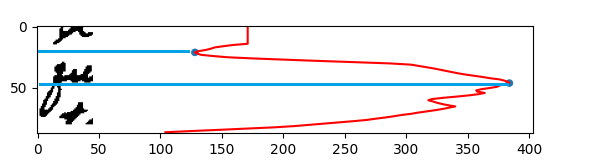
\includegraphics[width = 0.5\linewidth]{Figure_1.png}
                \caption{Segmento vertical de 5\% de imagen, en rojo el SPR y en azul los extremos del SPR, en el intermedio est\'a la zona de texto y en los bordes la zona de interlineado.}
            \end{figure}
        \subsection{Margen} 
        
            Para determinar el margen se pueden considerar tanto los m\'argenes superior e inferior como los m\'argenes laterales \cite{21}, para nuestro Dataset, como las im\'agenes son l\'ineas manuscritas no tiene sentido analizar los m\'argenes superior e inferior, por tanto solo 
            se clasifica el margen lateral izquierdo en cuanto a su ancho como: Margen ancho (BIG\_MARGIN) y margen estrecho (SMALL\_MARGIN). Para esto se analiz\'o el perfil de proyeccci\'on (PR) horizontal de cada im\'agen tomando el rango del PR desde el elemento 0 hasta que el valor del PR 
            sea mayo que una tolerancia espec\'ificada, es decir mientras que la densidad de p\'ixeles en el foreground para cada columna de la imagen sea menor que un valor relativo al largo de la iamgen. 

            \begin{figure}[!h]
                \centering
                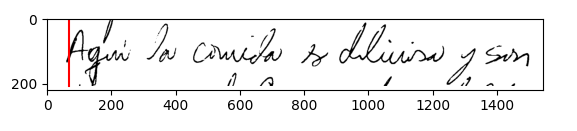
\includegraphics[width = 0.5\linewidth]{Margin.png}
                \caption{Desde el inicio hasta la l\'inea roja la secci\'on de margen.}
            \end{figure}
        \subsection{Espaciado} 

            El espaciado so los espacios dejados entre caracteres y palabras en una misma l\'inea, para clasificar el espaciado se realiz\'o a cada im\'agen un trabajo con filtros morfol\'ogicos, seleccionando un kernel horizontal para realizar una convoluci\'on con la imagen 
            que permita unificar los trazos de todo lo que est\'e escrito unido de una misma palabra para de este modo separar las palabras enmarc\'andolas en recuadros, as\'i el espaciado se puede determinar como la distancia promedio entre los recuadros.

            \begin{figure}[!h]
                \centering
                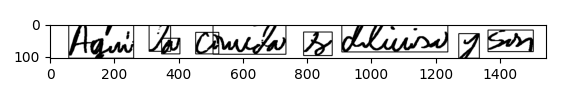
\includegraphics[width = 0.5\linewidth]{Espaces.png}
                \caption{Recuedros que bordean al texto escrito sin espacios.}
            \end{figure}

        \subsection{Inclinaci\'on de la L\'inea}
            Para determinar la inclinaci\'on de la letra en una l\'inea se realiz\'o el procedimiento descrito en \cite{20}, rotando la im\'agen desde $-30^{\circ}$ hasta $30^{\circ}$, 
            determinando para cu\'al de los valores de la rotaci\'on la cantidad de p\'ixeles de foreground es m\'axima para la zona central de la imagen. Para los \'angulos comprendidos 
            entre $ [-30; -5) $ se dice que la linea base es Ascendente (ASCENDING), entre $[-5; 5]$ es Nivelada (LEVELED) y entre $(5; 30]$ es Descendente (DESCENDING). 

            \begin{figure}[!h]
                \centering
                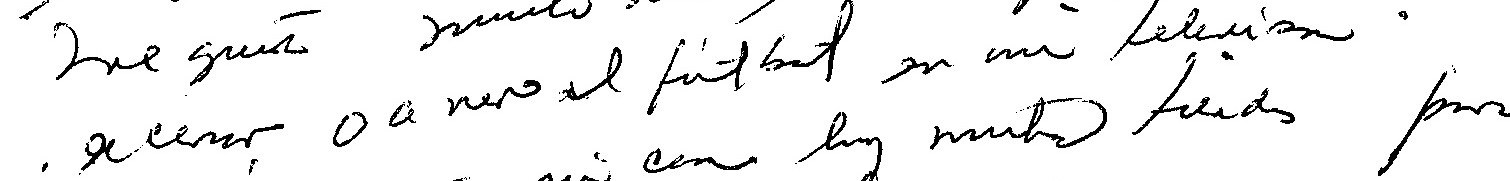
\includegraphics[width = 0.4\linewidth]{Judith_21.jpg}
                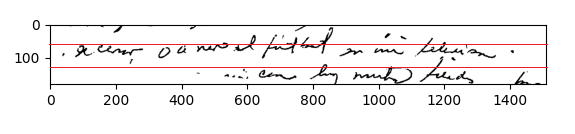
\includegraphics[width = 0.4\linewidth]{Baseline.png}
                \caption{a) texto original b) Texto con una inclinaci\'on de $-6^{\circ}$, la zona enmarcada en rojo es el \'area en que se busca maximizar 
                la cantidad de pixeles de foreground.}
            \end{figure}

        \subsection{Inclinaci\'on de la letra}
            Para la inclinaci\'on de la letra se tienen 5 posibles clasificaciones: Inclinado extremadamente a la izquierda (EXTREME\_LEFT), ligeramente inclinado a la 
            izquierda (MODERATE\_LEFT), as\'i como sus equivalentes hacia la derecha (EXTREME\_RIGHT) y (MODERATE\_RIGHT) respectivamente y la escritura sin inclinaciones (VERTICAL). 
            Para extraer este feature se utiliza el perfil de proyecci\'on (PR) vertical rotando la imagen en \'angulos entre $-20^{\circ}$ y $20^{\circ}$, buscando el \'angulo que maximice
            la suma del PR normalizado, tal y como se plantea en \cite{20}.
\section{Algoritmos Utilizados}
\subsection{KNN}
\subsection{CNN}
\subsection{K-Means}
\subsection{SVM}
\section{Resultados}

\begin{thebibliography}{99}
    %-----------------------------------------------------------------------------------
        \bibitem{1} \emph{International Conference on Computational Techniques, Electronics and Mechanical.} 2018. 
    
        \bibitem{2} \emph{Handwriting Analysis based on Histogram of Oriented Gradient for Predicting Personality traits using SVM.} Procedia Computer Science, vol. 165, 2019.
    
        \bibitem{3} \emph{Personality Prediction based on Handwriting using Machine Learning.}
        
        \bibitem{4} \emph{A framework for analyzing financial behavior using machine learning classification of personality through handwriting analysis.}
    
        \bibitem{5} \emph{E-Graphologist for Personality Profile.}

        \bibitem{6}  \emph{Personality Prediction System Based on Signatures}
        
        \bibitem{7}  \emph{Graphology for Farsi Handwriting Using Image Processing Techniques    }
        
        \bibitem{8}  \emph{A Framework for Determining the Big Five Personality Traits Using Machine Learning Classification through Graphology}
        
        \bibitem{9}  \emph{Personality analysis through handwriting recognition}
        
        \bibitem{10} \emph{Personality Type Assessment System by using  Enneagram-Graphology Techniques on Digital  Handwriting}
        
        \bibitem{11} \emph{Analysis of Signature for the Prediction of Personality\_Traits}
        
        \bibitem{12} \emph{Artificial Neural Network for Human Behavior Prediction  through Handwriting Analysis}
        
        \bibitem{13} \emph{EMOTHAW\_A\_novel\_database\_for\_emotional\_state\_recog}
        
        \bibitem{14} \emph{IEEE Xplore Full-Text PDF}
        
        \bibitem{15} \url{https://data.csafe.iastate.edu/DataPortal/#HandwritingDatabase} 
        
        \bibitem{16} \url{https://fki.tic.heia-fr.ch/databases/iam-handwriting-database} 

        \bibitem{17} \emph{Forensic Graphology Assessment of Personality}

        \bibitem{18} \emph{Handwriting Personality Recognition with Machine  Learning: A Comparative Study}

        \bibitem{19} \emph{GRAPHOLOGY: UNDERSTANDING – MISUNDERSTANDING.}

        \bibitem{20} \emph{Predicting the Big Five personality traits from handwriting } 2018

        \bibitem{21} \emph{A Machine Learning Approach to Employability Evaluation Using Handwriting Analysis}

        \bibitem{22} \emph{Handwritten document image segmentation into text lines and words} 2010
        
        \bibitem{23} \url{https://bigfive-test.com}
        %-----------------------------------------------------------------------------------
    \end{thebibliography}
\end{document}